\begin{figure}[htbp]
\centering
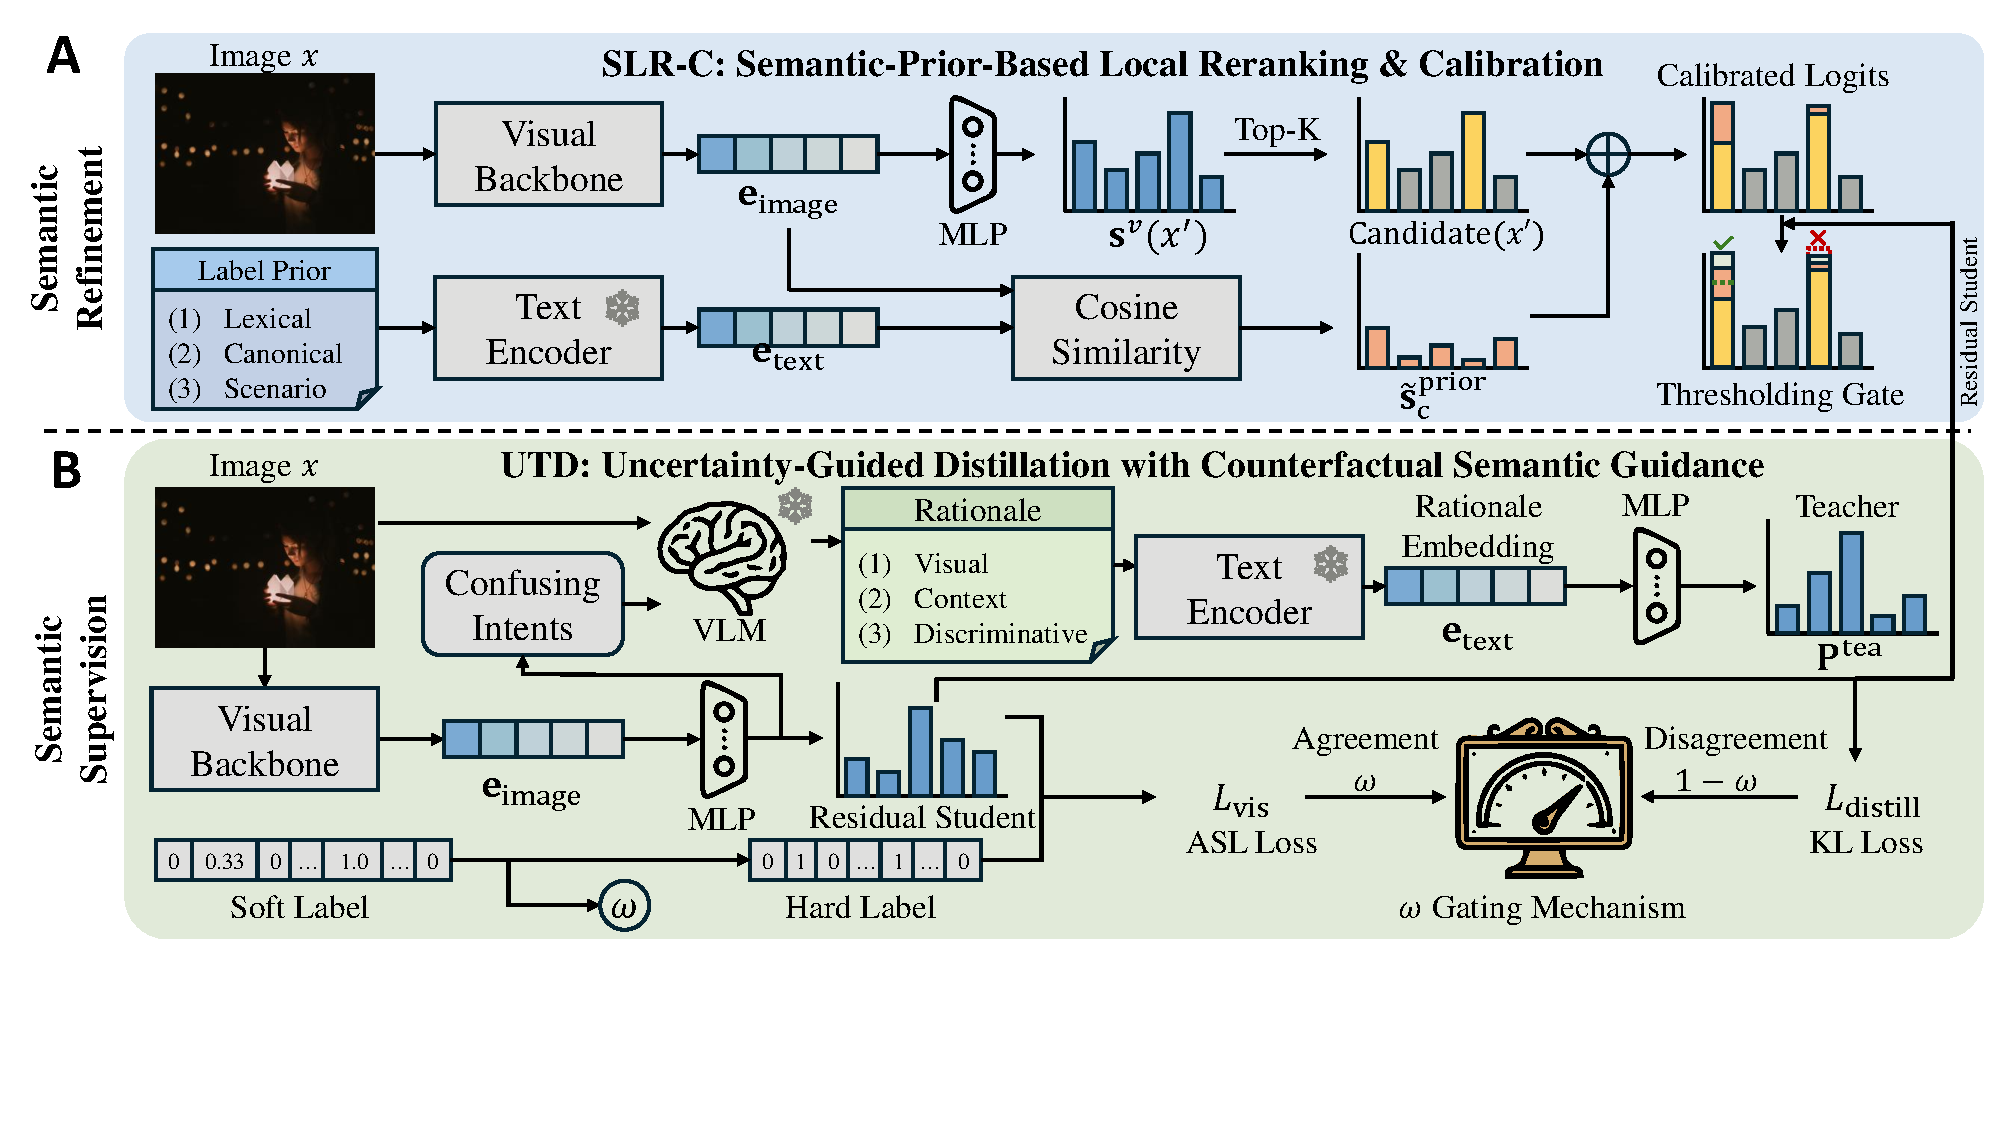
\includegraphics[width=\linewidth]{2_framework.pdf}
\caption{Overview of FDIL. SLR-C constructs a textual semantic prior and performs local reranking plus residual refinement. UTD uses a rationale-based text teacher and an agreement-aware gate to stabilize learning under ambiguous supervision.}
\label{fig:fdil_framework}
\end{figure}

\section{Method}
\label{sec:method}

\subsection{Overview}

To address the dual challenges of supervisory ambiguity and semantic ambiguity in visual intention recognition, we propose the \textbf{FDIL}, a functionally decoupled framework where fixed semantic priors provide structured candidate semantics, uncertainty-aware text teachers stabilize ambiguous supervision, and a residual student learns image-aware intent prediction on top of the semantic prior. Instead of forcing one unified mechanism to handle both supervisory ambiguity and semantic ambiguity, we assign them to two complementary functions.

FDIL consists of two key components, as shown in Figure~\ref{fig:fdil_framework}.
\begin{itemize}
    \item \textbf{Semantic Local Reranking and Calibration (SLR-C)}, which constructs a semantic prior from heterogeneous textual cues and supports image-aware refinement through a residual student.
    \item \textbf{Uncertainty-guided Text Distillation (UTD)}, which introduces adaptive semantic guidance to improve robustness under ambiguous supervision.
\end{itemize}

Given an input image, the model first produces visual intent scores using a strong visual backbone. SLR-C then provides structured candidate semantics by locally reranking intent candidates and forming a semantic prior. UTD supplies uncertainty-aware semantic supervision through a rationale-based text teacher and can be reused to regularize both the visual student and the residual refinement module built on top of the semantic prior.

%% --- BEGIN condensed-out for page limit: notation table removed; every symbol
%% is now defined inline at its first occurrence in the text. ---
\iffalse
\begin{table}[htbp]
\centering
\small
\caption{Key notation used in the method.}
\label{tab:notation}
\setlength{\tabcolsep}{6pt}

\begin{tabular}{ll}
\hline
Symbol & Meaning \\
\hline
$x$ & input image \\
$\mathcal{Y},\,C$ & intent label space and number of classes \\
$\mathbf{y}^{\text{soft}},\,\mathbf{y}^{\text{hard}}$ & soft annotation / binarized hard labels \\
$\omega\in(0,1]$ & sample-level annotator agreement score \\
$\phi=f_{\text{img}}(x)$ & frozen visual image feature \\
$\tilde{s}^{\text{prior}}_c$ & normalized heterogeneous semantic prior \\
$\mathcal{C}_K(x),\,K$ & Top-$K$ candidate set and its size \\
$s^{\text{full}}_c$ & final refined score for class $c$ \\
$t_c$ & class-wise decision threshold (validation-only) \\
$\mathbf{p}^{\text{tea}},\,\tau$ & text-teacher distribution and temperature \\
$g=1-\omega$ & teacher-branch gate weight \\
$\mathcal{L}_{\text{total}}$ & total training loss \\
\hline
\end{tabular}

\end{table}
\fi
%% --- END condensed-out ---

\subsection{Problem Formulation}

Given an input image $x$, the goal is to predict a set of intent labels from a predefined label space $\mathcal{Y}=\{1,\dots,C\}$, where $C$ is the total number of intent categories. Due to the subjective nature of visual intention recognition, annotations are provided as soft label vectors $\mathbf{y}^{\text{soft}} \in \{0, 0.33, 0.66, 1\}^C$, reflecting annotator agreement.

Existing approaches typically follow either hard binarization or soft regression paradigms, both of which have limitations under ambiguous supervision. To address this, we adopt a \textbf{decoupled utilization} of annotation signals.

Specifically, we derive binarized labels $\mathbf{y}^{\text{hard}}$ for classification supervision, while extracting an image-level agreement score $\omega \in (0,1]$ from $\mathbf{y}^{\text{soft}}$. Here, $\omega$ reflects annotator consensus, where higher values indicate more reliable supervision. The binarized labels are computed as.
\begin{equation}
y^{\text{hard}}_{c} =
\begin{cases}
1, & \text{if } y^{\text{soft}}_{c} > 0 \\
0, & \text{otherwise}
\end{cases}
\end{equation}

In practice, an image may contain multiple positive intents with different agreement levels. We therefore adopt a conservative pooling rule and define the sample-level agreement as the minimum soft agreement among all positive labels.
\begin{equation}
\omega = \min_{c:\, y^{\text{hard}}_{c}=1} y^{\text{soft}}_{c}.
\end{equation}
This choice lets the hardest positive label determine how much the sample should trust direct supervision.

\subsection{Semantic Local Reranking and Calibration (SLR-C)}

Semantic ambiguity mainly manifests as local confusion among visually plausible but semantically adjacent intents. A candidate-recall diagnostic shows that the baseline Top-10 candidates already cover $83.9\%$ of positive labels, and $67.8\%$ of its false negatives remain recoverable within this set. This suggests that many errors arise from ranking confusable intents rather than failing to retrieve the correct intent. To address this, we build a semantic refinement module that provides structured candidate semantics before turning to ambiguity-aware supervision.

\subsubsection{Semantic Prior Construction}

Intent semantics are inherently multi-granular and abstract, making a single textual representation insufficient. We therefore construct a heterogeneous semantic prior for each intent by combining three complementary textual sources, namely lexical intent phrases, canonical intent descriptions, and descriptive visual scenarios. The lexical source provides concise intent name cues, the canonical source provides semantic definitions, and the scenario source grounds abstract intents into plausible visual situations.

\paragraph{Example}
For the intent \textit{SocialLifeFriendship}, the lexical phrase is \textit{``Social Life and Friendship''}, and the canonical description is.
\textit{``Being part of a social group. Having people to do things with. Having close friends, others to rely on. Making friends, drawing others near.''}
This intent is further expanded into multiple scenario archetypes with distinct visual realizations. For \textit{SocialLifeFriendship}, scenarios include friends hiking together, close friends talking on a couch, a group dinner, or volunteers gardening together.

%% --- BEGIN condensed-out for 35-page limit (full scenario examples retained below) ---
\iffalse
\begin{quote}
\small
\textbf{Scenario 1}
\textit{``A photo of a group of friends hiking up a steep mountain trail together, wearing backpacks, laughing and giving high-fives under a bright sunny sky.''}

\textbf{Scenario 2}
\textit{``An image showing two close friends sitting on a comfortable living room couch, drinking coffee, leaning in closely to share a deep, supportive conversation.''}

\textbf{Scenario 3:}
\textit{``A photo of a large group of diverse people gathered around a busy dinner table, laughing loudly and toasting glasses of wine in a warmly lit room.''}

\textbf{Scenario 4:}
\textit{``An image showing a group of cheerful volunteers working together in a lush community garden, planting flowers side-by-side with dirty hands and bright smiles.''}
\end{quote}
\fi
%% --- END condensed-out for 35-page limit ---

The scenarios are not hand-picked but produced by a fixed generation protocol applied uniformly to every intent class (template released with our artifacts), under which the vision-language model enumerates visually distinct realizations along five axes (subjects/objects, actions, settings, atmosphere, and photographic style), with at least three settings per intent so as to span intra-class variation rather than a single canonical view. Inclusion favors representativeness over exhaustive coverage. Outside the generated scenarios the prior degrades gracefully toward the lexical and canonical sources, the base logits, and the residual student.

Given an image $x$, we score each intent by the CLIP-scaled cosine similarity between the image feature $f_{\text{img}}(x)$ and the text embedding $\mathbf{e}_c$ of class $c$.
\begin{equation}
s^{\text{prior}}_c = \text{sim}(f_{\text{img}}(x), \mathbf{e}_c) = \gamma \cdot \frac{f_{\text{img}}(x)^\top \mathbf{e}_c}{\|f_{\text{img}}(x)\|_2 \|\mathbf{e}_c\|_2},
\end{equation}
where $\gamma$ is the CLIP logit scale. Each source $r \in \{\text{lex}, \text{can}, \text{scen}\}$ is normalized independently across the $C$ classes and the three are averaged into the prior.
\begin{equation}
\tilde{s}^{r}_c = \frac{s^{r}_c - \mu^{r}(x)}{\sigma^{r}(x) + \epsilon},
\qquad
\tilde{s}^{\text{prior}}_c = \frac{1}{3}\sum_{r}\tilde{s}^{r}_c,
\end{equation}
where $\mu^{r}(x)$ and $\sigma^{r}(x)$ are the per-sample mean and standard deviation over the $C$ intent classes and $\epsilon$ ensures numerical stability.

\subsubsection{Semantic Local Reranking}

In the refinement module, we start from base visual logits $\mathbf{s}^{b}$ produced by a frozen visual student. We first select a compact candidate set as.
\begin{equation}
\mathcal{C}_K(x) = \text{TopK}(\mathbf{s}^{b}, K).
\end{equation}
The base logits are then locally adjusted with the normalized prior.
\begin{equation}
\tilde{s}_c =
\begin{cases}
s^{b}_c + \alpha \cdot \tilde{s}^{\text{prior}}_c, & c \in \mathcal{C}_K(x), \\
s^{b}_c, & \text{otherwise}.
\end{cases}
\end{equation}
Here $\alpha$ controls the strength of semantic reranking. In our implementation, $\alpha$ is fixed to 0.3.

This localized reranking produces a semantic prior that narrows the candidate set and sharpens the local score geometry without introducing an additional trainable prior module.

\subsubsection{Residual Refinement on the Semantic Prior}

Fixed reranking alone is not sufficient, because the heterogeneous prior may still fall short of the image-specific evidence. We therefore train a lightweight residual student on top of the semantic prior.
\begin{equation}
s^{\text{full}}_c = \tilde{s}_c + h_{\text{res}}(f_{\text{img}}(x))_c,
\end{equation}
where $h_{\text{res}}(\cdot)$ is a residual MLP that predicts class-wise residual intent scores from the image feature. In practice, the SLR-C logits $\tilde{s}_c$ are first computed and frozen, and the residual module is then optimized separately.

In the final full model, this residual module is not trained in isolation, since it can also be regularized by the uncertainty-aware text teacher introduced next. Thus, SLR-C provides the structured candidate semantics first, and UTD later supplies the ambiguity-aware supervision used to stabilize image-aware prediction on top of the semantic prior.

\subsubsection{Class-wise Calibration}

Motivated by Guo et al. \cite{guo_calibration_2017}, to account for class imbalance and varying score distributions, we adopt class-wise thresholds.
\begin{equation}
\hat{y}_c = \mathbb{I}[\sigma(s^{\text{full}}_c) > t_c],
\end{equation}
where $t_c$ is determined on the validation set. Concretely, each threshold is selected independently by maximizing the class-wise validation F1 score.
\begin{equation}
t_c^\ast = \arg\max_{t \in \mathcal{T}} \text{F1}_c^{\text{val}}(t),
\end{equation}
where $\mathcal{T}$ is a fixed threshold grid. This design lets each class adapt its decision boundary to its own score distribution and frequency level, instead of sharing a single global threshold.

\subsection{Uncertainty-guided Text Distillation (UTD)}

%\subsubsection{Motivation}

Supervisory ambiguity arises when multiple plausible intents coexist for a given image. Direct optimization against hard labels may lead to overconfident predictions and unstable decision boundaries. To alleviate this issue, we introduce semantic guidance from text space and adapt its influence based on the uncertainty of supervision.

\subsubsection{Text-derived Teacher}

For each training image, we construct structured textual descriptions that capture semantic cues relevant to intention understanding. These descriptions are generated offline by a vision-language model, guided by both the image content and intent semantics.

To enhance discriminative capability under semantic ambiguity, we further incorporate contrastive cues by identifying visually plausible but incorrect intents predicted by the current model. Specifically, we select high-confidence negative intents as confusion candidates and use them to guide the generation of discriminative textual descriptions. This encourages the resulting text to emphasize subtle distinctions among semantically adjacent intents.

The generated text aims to summarize three aspects.
(1) observable visual elements,
(2) contextual interpretation beyond direct perception, and
(3) discriminative cues for distinguishing confusing intents.

The resulting text $T(x)$ is encoded into a dense embedding space using a frozen text encoder.
\begin{equation}
\mathbf{e}_{\text{text}} = f_{\text{text}}(T(x)).
\end{equation}

A lightweight classifier then maps the embedding into a multi-label teacher distribution.
\begin{equation}
\mathbf{p}^{\text{tea}} = \sigma(g_{\text{tea}}(\mathbf{e}_{\text{text}}) / \tau),
\end{equation}
where $\sigma(\cdot)$ is the sigmoid function and $\tau$ is the temperature parameter.

This design introduces contrastive semantic signals that improve the teacher's ability to distinguish semantically similar intents, while remaining separate from the semantic prior itself. In the full FDIL pipeline, the same teacher can further regularize the residual refinement module built on top of SLR-C.

\subsubsection{Uncertainty-guided Distillation}

The visual backbone produces logits $\mathbf{s}^{v}$ for image $x$. We adopt the Asymmetric Loss \cite{ridnik_asymmetric_2021} for classification.
\begin{equation}
\mathcal{L}_{\text{vis}} = \frac{1}{C} \sum_{c=1}^{C} \ell_{\text{ASL}}(s^{v}_{c}, y^{\text{hard}}_{c}).
\end{equation}

To incorporate semantic guidance, we introduce an uncertainty-guided Bernoulli distillation loss.
\begin{equation}
\mathcal{L}_{\text{distill}} = \sum_{c=1}^{C}\text{KL}\big(\mathrm{Bern}(p_c^{\text{tea}})\,\|\, \mathrm{Bern}(\sigma(s_c^{v}/\tau))\big),
\end{equation}
which is applied independently to each label. We use Bernoulli-style distillation rather than softmax distillation because intent recognition is a multi-label problem in which each intent is modeled as an independent Bernoulli variable rather than as a mutually exclusive class on a probability simplex. This formulation preserves per-class uncertainty and avoids imposing artificial competition among labels.

Rather than mixing the two objectives with a fixed global coefficient, we use a gate derived from the agreement score. For the current sample, the teacher branch weight is defined as $g = 1 - \omega$, so low-agreement samples receive stronger semantic guidance, while high-agreement samples remain dominated by direct visual supervision.

Using $g$, the final loss is defined as.
\begin{equation}
\mathcal{L}_{\text{total}} = (1-g)\mathcal{L}_{\text{vis}} + \lambda g \mathcal{L}_{\text{distill}}
= \omega \mathcal{L}_{\text{vis}} + \lambda (1-\omega)\mathcal{L}_{\text{distill}},
\end{equation}
where $\lambda$ is the distillation loss weight.

This gated formulation allows the model to rely more on visual supervision when annotations are reliable, and to leverage semantic guidance when supervision is uncertain. In other words, UTD stabilizes ambiguous supervision through an uncertainty-aware text teacher rather than by modifying the semantic prior itself.

\subsection{Functionally Decoupled Ambiguity Modeling}
\label{sec:decoupling_principle}

We interpret visual intention recognition as a functionally decoupled ambiguity problem, formed by semantic confusion among neighboring intents and supervisory uncertainty from subjective annotations.

\revised{\textbf{Two ambiguities, two learning problems.}
Let $X$ denote the image, $Z=\phi(X)$ its deterministic visual representation, and $Y_c\in\{0,1\}$ a random human judgement for intent $c$. Then
\begin{equation}
\label{eq:entropy_decomp}
H(Y_c\mid Z)
=
\underbrace{H(Y_c\mid X)}_{\text{irreducible supervisory}}
+
\underbrace{I(Y_c;X\mid Z)}_{\text{discarded by }\phi} ,
\end{equation}
which follows from
$I(Y_c;X\mid Z)=H(Y_c\mid Z)-H(Y_c\mid X,Z)$ and
$H(Y_c\mid X,Z)=H(Y_c\mid X)$ because $Z=\phi(X)$.
The first term is disagreement persisting given the complete image. Being a functional of the annotation distribution $\Pr(Y_c\mid X)$ alone, it cannot be reduced by any choice of $\phi$ or any predictor reading $Z$. The second is label-relevant information that $X$ carries but $Z$ discards, a functional of the representation map. \eqref{eq:entropy_decomp} serves to show that the two deficits are functionals of different objects and hence pose two learning problems, what the model is asked to fit and what information the decision rule can access, which is why FDIL treats them with mechanisms of different type.}

\revised{\textbf{SLR-C supplies label-relevant information the baseline underuses.}
Let $B=\mathbf{s}^{b}(Z)$ be the baseline logits and $S=\tilde{\mathbf{s}}^{\mathrm{prior}}(X)$ the text-side prior scores. Since $B$ is a function of $Z$, the data-processing inequality gives $H(Y_c\mid B)\ge H(Y_c\mid Z)$, showing that the baseline prediction is in general insufficient, retaining only part of the label-relevant information. Conditioning additionally on the prior gives the  identity
\begin{equation}
\label{eq:cmi_prior}
H(Y_c\mid B,S)=H(Y_c\mid B)-I(Y_c;S\mid B),
\end{equation}
so residual uncertainty falls by the conditional mutual information $I(Y_c;S\mid B)$, the label-relevant information in the prior that the baseline prediction does not already carry, which is zero precisely when $S$ is redundant given $B$. SLR-C is therefore an injection of under-used text-side information, and $\tilde{s}_c=s^{b}_c+\alpha\tilde{s}^{\mathrm{prior}}_c$ is the minimal way to make the decision rule a function of $(B,S)$ rather than of $B$ alone.}

\revised{\textbf{Top-$K$ reranking as local hypothesis screening.}
For a positive intent $c^+$ and a confusing intent $c^-$ in $\mathcal{C}_K(x)$, let
$m=s^b_{c^+}-s^b_{c^-}$ and
$\Delta_{\mathrm{prior}}
=\tilde{s}^{\mathrm{prior}}_{c^+}
-\tilde{s}^{\mathrm{prior}}_{c^-}$, and the reranking rule gives
\begin{equation}
\label{eq:margin_identity}
m'-m=\alpha\Delta_{\mathrm{prior}},
\end{equation}
so the margin grows whenever the prior ranks $c^+$ above $c^-$, a reversed pair is corrected when $\alpha\Delta_{\mathrm{prior}}\ge -m>0$, and scores outside $\mathcal{C}_K(x)$ are untouched. Restricting the prior to $\mathcal{C}_K(x)$ is thus local hypothesis screening, in the sense of variable screening for high-dimensional selection. The semantic channel acts only on hypotheses the visual evidence already deems plausible. $K$ balances coverage against distractor noise. SLR-C therefore does not globally rescore the label space but corrects semantic confusion among high-probability candidates.}

\revised{\textbf{UTD as reliability-weighted privileged information.}
The rationale teacher reads a textual description $T(x)$ generated with access to intent semantics and model-specific confusion candidates, which exists at training time only. UTD therefore uses privileged information \cite{vapnik_new_2009}, realized through distillation \cite{lopez-paz_unifying_2016}, and must decide how much to trust that privileged channel. In a per-sample scalar view of one label, the annotated target is $y_v=y+\varepsilon_v$ with $\mathbb{E}\varepsilon_v=0$ and $\mathrm{Var}(\varepsilon_v)=\sigma_v^2(\omega)$, decreasing in the agreement score $\omega$ since higher consensus means less annotation noise, while the teacher gives $y_t=y+b_t+\varepsilon_t$ with bias $b_t$ and independent noise of variance $\sigma_t^2$. For $\hat{y}(g)=(1-g)y_v+g\,y_t$ we have $\mathrm{MSE}(g)=(1-g)^2\sigma_v^2(\omega)+g^2(\sigma_t^2+b_t^2)$, minimized at
\begin{equation}
\label{eq:opt_gate}
g^{\ast}
=
\frac{\sigma_v^2(\omega)}
{\sigma_v^2(\omega)+\sigma_t^2+b_t^2},
\end{equation}
which increases with supervision noise, decreases with teacher noise and bias, and is monotonically decreasing in $\omega$. Our gate $g=1-\omega$ is a monotone, parameter-free approximation of \eqref{eq:opt_gate}. It keeps the correct direction without estimating $\sigma_t^2$ or $b_t^2$, and reaches $g=0$ at $\omega=1$, where supervision is effectively noiseless and the privileged channel can only add bias. The teacher contribution to the student-logit gradient is then
\begin{equation}
\label{eq:gate_grad}
\frac{\partial\,\lambda(1-\omega)\mathcal{L}_{\mathrm{distill}}}
{\partial s^v_c}
=
\frac{\lambda(1-\omega)}{\tau}(p_c-q_c),
\end{equation}
with $p_c=\sigma(s^v_c/\tau)$ and $q_c=p^{\mathrm{tea}}_c$, so guidance is routed in proportion to annotator disagreement.}

\revised{In summary, SLR-C addresses prediction-semantic insufficiency in the decision space, while UTD addresses unreliable supervision through uncertainty-weighted privileged information. Since each module is tied to a different deficit, their gains should be distinctly sensitive to the two ambiguity sources, which we test in Sec.~\ref{sec:quadrants}.}
